\section*{Motivation}
Viele Menschen mit k�rperlicher Behinderung sind auf pers�nliche Assistenz angewiesen. Diese Assistenz umfasst neben der Pflege auch die Erf�llung allt�glicher Aufgaben. Mit Hilfe pers�nlicher Assistenz wird ein selbstbestimmtes Leben erm�glicht. 

In dieser Ausarbeitung wird ein k�rperlich behinderter Mensch (im folgenden \enquote{Klient} genannt) herausgegriffen. Dieser Klient hat sieben Assistenten. Die Verwaltung geschieht �ber einen Dienstplan. Bisher erstellte der Klient den Dienstplan jeden Monat manuell. Der Klient hat gleichzeitig die sieben E-Mails seiner Assistenten �berblickt (in denen m�gliche Arbeits-Termine enthalten waren) und einen m�glichst ausgewogenen Dienstplan erstellt. Der Dienstplan sollte die Verf�gbarkeiten und die Stundenkontingente der Assistenten m�glichst gut ber�cksichtigen. Das manuelle Erstellen des Dienstplans dauerte ca. vier Stunden pro Monat.

Um den Klienten zu entlasten und technisch besser zu unterst�tzen, wurde die Idee des Assistenzplaners ins Leben gerufen. Der Assistenzplaner soll als serverbasierte Anwendung den Klienten und sein Team bei der Dienstplanerstellung unterst�tzen. Der Klient und alle Assistenten erhalten einen personalisierten Zugang zum Assistenzplaner und k�nnen alle n�tigen Informationen austauschen. Ein Algorithmus erstellt den Dienstplan unter Ber�cksichtigung aller Vorlieben des Klienten und der Stundenkontingente der Assistenten. Der Zeitaufwand f�r die Dienstplanerstellung sollte auf wenige Minuten sinken.

\section*{Anforderungsermittlung}
Die Anforderungen wurden zum einen als Benutzergeschichten festgehalten. Weiterhin wurden Anforderungen formuliert, die zwar vom Benutzer nicht explizit erw�hnt wurden, jedoch trotzdem f�r den Assistenzplaner essenziell waren.\\[1ex]

Die Anforderungen wurden in SysML modelliert. Ein beispielhaftes Anforderungsdiagramm ist in Abbildung \ref{fig:SysMLRequirementsRoster} dargestellt.\\[1ex]

\begin{figure}[H]
	\centering
	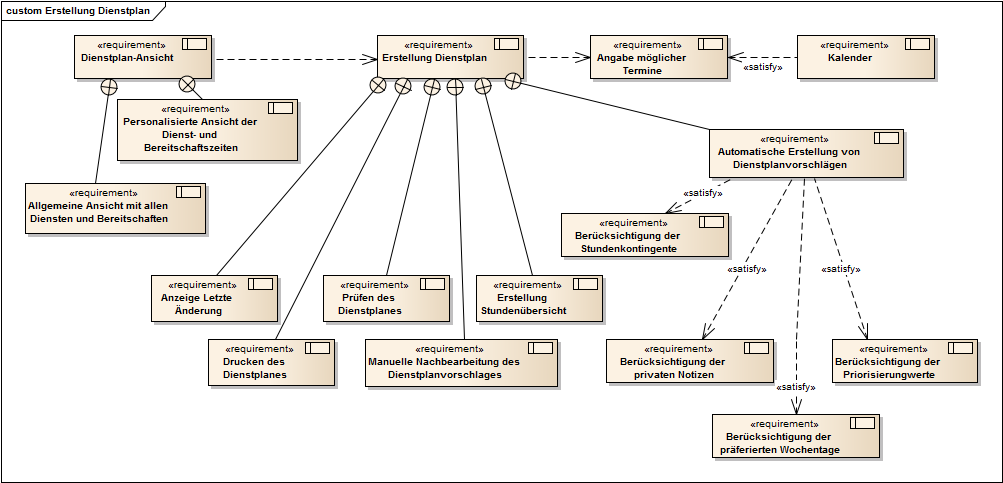
\includegraphics[width=1.0\textwidth]{../Images/Modell/SysMLRequirementsRoster.png}
	\caption{SysML Anforderungsdiagramm - Bereich Dienstplan}
	\label{fig:SysMLRequirementsRoster}
\end{figure}